\section{整数规划}
\subsection{整数规划}
整数规划就是线性规划加上解必须为整数的限制,其基本形式为
$$
\max \quad c^Tx
$$
$$
\text{s.t.} 
\begin{cases}
    Ax \le b \\
    x \in \mathbb{N}
\end{cases}
$$
常见的很多算法问题都能写成线性整数规划的形式,特别是能写成整数规划的一种特殊形式:$0 - 1$ 规划。

\subsubsection{$0 - 1$ 背包问题}
假设共有 $n$ 件物品,$v_i$ 表示第 $i$ 件物品的价值,$w_i$ 表示第 $i$ 件物品的重量,$c$ 表示背包的最大承重,$x_i \in \{0, 1\}$ 表示是否选择第 $i$ 件物品。 $0-1$ 背包问题可以写为
$$
\max \quad v_ix_i
$$
$$
\text{s.t.} 
\begin{cases}
    \sum_{i = 1}^n w_ix_i \le c \\
    x \in \{0, 1\}
\end{cases}
$$

\subsubsection{最小生成树问题}
假设共有 $n$ 个点,点集为 $V$,$(i, j) \in E$ 表示从第 $i$ 个点连到第 $j$ 个点的一条有向边,$w_{i, j}$ 表示边的权重,$x_{i, j} \in \{0, 1\}$ 表示这一条边是否在最小生成树内。最小生成树问题可以写为 \\
$$
\min \quad \sum_{(i, j) \in E} w_{i, j}x_{i, j}
$$
$$
\text{s.t.} 
\begin{cases}
    \sum_{(i, j) \in E} x_{i, j} = n - 1 \\
    \sum_{i \in S, j \notin S} x_{i, j} \ge 1, \ \forall S \subset V, \ S \ne V\\
    x_{i, j} \in \{0, 1\}
\end{cases}
$$

\subsubsection{装箱问题}
假设共有 $n$ 个物品,$w_i$ 表示第 $i$ 个物品的重量,$c$ 表示每个箱子的承重,$x_{i, j} \in \{0, 1\}$ 表示是否将第 $i$ 个物品放入第 $j$ 个箱子,$y_i$ 表示是否使用第 $i$ 个箱子。装箱问题可以写为
$$
\min \quad \sum_{i = 1}^n y_i
$$
$$
\text{s.t.} 
\begin{cases}
    \sum_{i = 1}^n w_ix_{i, j} \le cy_i, \ \forall j \in \{1, 2, \ \cdots, n\} \\
    \sum_{j = 1}^n x_{i, j} = 1, \ \forall i \in \{1, 2, \ \cdots, n\} \\
    x_{i, j} \in \{0, 1\} \\
    y_{i, j} \in \{0, 1\} 
\end{cases}
$$

\subsubsection{匹配问题}
假设图的点集为 $V$,边集为 $E$。设 $(i, j) \in E$ 表示从第 $i$ 个点连到第 $j$ 个点的一条有向边,$x_{i, j}$ 表示这条边是否为匹配边。一般无向图的最大匹配问题可以写为
$$
\min \quad \sum_{(i, j) \in E} x_{i, j}
$$
$$
\text{s.t.} 
\begin{cases}
    \sum_{(i, j) \in E} x_{i, j} \le 1, \ \forall i \in V \\
    \sum_{(i, j) \in E} x_{i, j} \le 1, \ \forall j \in V \\
    x_{i, j} \in \{0, 1\}
\end{cases}
$$

\subsection{割平面法}
Gomory 割平面法 (Gomory cutting-plane method)是一种解线性整数规划问题的方法,思想就是一直去除非整数的最优解,直到某一次求得的最优解为整数。 \\
考虑一个线性规划问题,假设使用单纯形表求解后获得的不是整数解,可以选择一个非整数的变量 $x_i$,根据单纯形表有
\begin{align}
    x_i + \sum_{j = n + 1}^n \bar{a_{i, j}}x_j = \bar{b_i} \tag{1}
\end{align}
既然 $x_i$ 不是整数,说明 $\bar{b_i}$ 一定不是整数,当然 $\bar{a_{i, j}}$ 也可能不是整数。调整 $(1)$。
\begin{align}
    x_i + \sum_{j = n + 1}^n \left\lfloor \bar{a_{i, j}} \right\rfloor x_j \le \bar{b_i} \tag{2}
\end{align}
$(1)$ 一定是 $(2)$ 的解。调整 $(2)$
\begin{align}
    x_i + \sum_{j = n + 1}^n \left\lfloor \bar{a_{i, j}} \right\rfloor x_j \le \left\lfloor \bar{b_i} \right\rfloor \tag{3}
\end{align}
$(2)$ 的整数解一定符合 $(3)$,若用单纯形表求出的非整数解就不符合 $(3)$。只要把式$(3)$加入原来的线性规划问题,重新求解多出一个限制的线性规划问题。如果求出来的是整数解就停止,否则继续加入限制并求解,直到获得整数解为止。 \\
改变 $(3)$,变为 $(1) - (3)$
\begin{align}
    x_i + \sum_{j = n + 1}^n (\bar{a_{i, j}} - \left\lfloor \bar{a_{i, j}} \right\rfloor) x_j \ge \bar{b_i} - \left\lfloor \bar{b_i} \right\rfloor \tag{3}
\end{align}
假设有以下问题:
$$
\max \quad 3x_1 + 2x_2
$$
$$
\text{s.t.} 
\begin{cases}
    2x_1 + 3x_2 + x_3 = 14 \\
    2x_1 + x_2 + x_4 = 9 \\
    x \ge 0
\end{cases}
$$
有最终单纯形表
$$
\begin{array}{c|cccc|c} & 0 & 0 & -1/4 & -5/4 & -59/4 \\ \hline x_2 & 0 & 1 & 1/2 & -1/2 & 5/2 \\ x_1 & 1 & 0 & -1/4 & 3/4 & 13/4 \end{array}
$$
选择 $x_2$,加入限制:$x_2 - x_4 \le 2$,即 $x_2 - x_4 + x_5 = 2$。用单纯形表求解加入限制后的问题,得到最终单纯形表
$$
\begin{array}{c|ccccc|c} & 0 & 0 & 0 & -1 & -1/2 & -29/2 \\ \hline x_3 & 0 & 0 & 1 & 1 & -2 & 1 \\ x_1 & 1 & 0 & 0 & 1 & -1/2 & 7/2 \\ x_2 & 0 & 1 & 0 & -1 & 1 & 2 \end{array}
$$
选择 $x_1$,加入限制:$x_1 + x_4 - x_5 \le 3$,即 $x_1 + x_4 - x_5 + x_6 = 3$. 用单纯形表求解加入限制后的问题,得到最终单纯形表
$$
\begin{array}{c|cccccc|c} & 0 & 0 & 0 & -1 & 0 & -1 & -14 \\ \hline x_3 & 0 & 0 & 1 & 1 & 0 & -4 & 3 \\ x_1 & 1 & 0 & 0 & 1 & 0 & -1 & 4 \\ x_5 & 0 & 0 & 0 & 0 & 1 & -2 & 1 \\ x_2 & 0 & 1 & 0 & -1 & 0 & 2 & 1 \end{array}
$$
得到原问题的最优解为$x_1 = 4, x_2 = 1$​,目标函数值为 $14$。

\subsection{分支定界法}
将原问题放松成线性规划问题,解这个线性规划,得到了整数规划最优解的上界。假设最优解中 $N < x_i < N + 1$ 不是整数,此时有两种可能:$x_i \le N$ 或 $x_i \ge N+1$,对两种情况分别进行搜索。如果在某一枝算出了一个整数解,就得到了原整数规划最优解的下界;如果在另一枝线性规划问题的解没有比这个下界更优,则那一枝可以直接不考虑了(因为线性规划问题的解是那一枝能找到的最优解的上界)。 \\~\\
假设有以下问题:
\begin{figure}[H]
    \begin{center}
        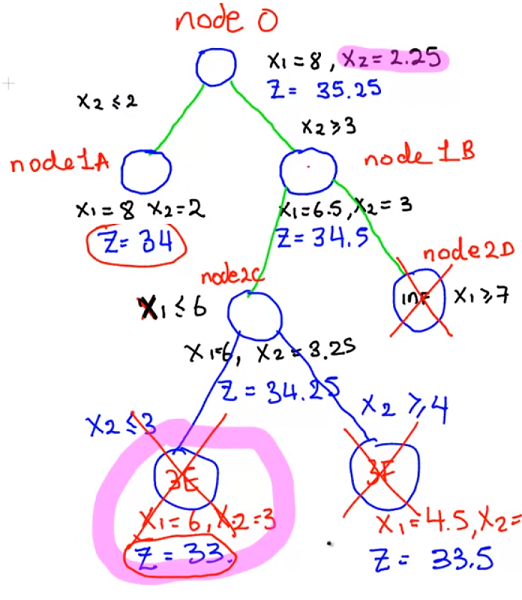
\includegraphics[scale=0.7]{img/branch_and_bound.png}
        \caption{分支定界法例子。}
    \end{center}
\end{figure}
\pagebreak
\begin{enumerate}
    \item 首先考虑 $x_2 \le 2$,也就是 node1A,算得该情况下最优解为 $x_1 = 8, x_2 = 2$,目标函数值为 $34$。这是一个整数解,记录并回溯。
    \item 考虑 $x_2 \ge 3$,也就是 node1B,算得该情况下的最优解为 $x_1 = 6.5, x_2 = 3$,目标函数值为 $34.5$。它还优于我们已知的下界 34,继续搜索。
    \item 考虑 $x_1 \le 6$,也就是 node2C,算得该情况下的最优解为 $x_1 = 6, x_2 = 3.25$,目标函数值为 $34.25$。它还优于我们已知的下界 34,继续搜索。
    \item 考虑 $x_2 \le 3$,也就是 node3E,算得该情况下的最优解为 $x_1 = 6, x_2 = 3$,目标函数值为 $33$。它劣于我们已知的下界 34,回溯。
    \item 考虑 $x_2 \ge 4$,也就是 node3F,算得该情况下的目标函数值为 $33.5$。它劣于我们已知的下界 $34$,回溯。
    \item 考虑 $x_1 \ge 7$,也就是 node2D,该情况下无可行解,回溯。
\end{enumerate}
搜索得最优解为 $x_1 = 8, x_2 = 2$,目标函数值为 $34$。

\pagebreak
